We therefore repriced the four scenario options under five IV variants on identical stock paths and found that the IV update changed option values before expiration and the lower tail of early-closing P\&L (Fig.~\ref{fig:dynamic_ablation}; Supplementary Table~\ref{tab:dynamic_ablation}). The variants ranged from frozen IV to the full factor, and we measured each against the direct surface on the same paths. Contracts, entry premiums, and pricing assumptions stayed fixed, so any price difference came from the IV update. After ten trading days, the full factor's prices differed from those of the direct surface by a mean absolute \$1.77--\$2.41 per share across the four options. These mean absolute differences were similar across the three evaluation seeds (Supplementary Table~\ref{tab:ablation_seeds}). For the GS put, the \$1.77 mean absolute change was about 38 times the \$0.047 decrease in mean P\&L. That decrease had a paired Monte Carlo standard error of \$0.04. Positive and negative differences therefore largely canceled across paths. Frozen IV and deterministic mean reversion also gave prices that differed from the direct surface. The moving target, and the lag with which the factor followed it, thus affected prices even without random shocks. Comparing the full factor with the uncoupled stochastic factor on the same paths isolated the effect of linking IV shocks to stock returns (Fig.~\ref{fig:dynamic_ablation}). For both tickers, short-put P\&L declined most on falling-stock paths, and short-call P\&L improved most on rising-stock paths. Coupling also changed the lower tail of short-position P\&L. We measured this tail by the 5\% expected shortfall, where more negative values mean larger losses. Negative coupling moved the GS put's expected shortfall from $-\$62.98$ under the uncoupled factor to $-\$64.60$ under the full factor. The GS call's expected shortfall improved from $-\$71.53$ to $-\$69.82$. The LLY options moved in the same directions (Supplementary Table~\ref{tab:dynamic_ablation}). All variants gave identical entry prices and payoffs at expiration, so an analysis of payoffs at expiration alone would have missed these differences.

\begin{figure}[H]
\centering
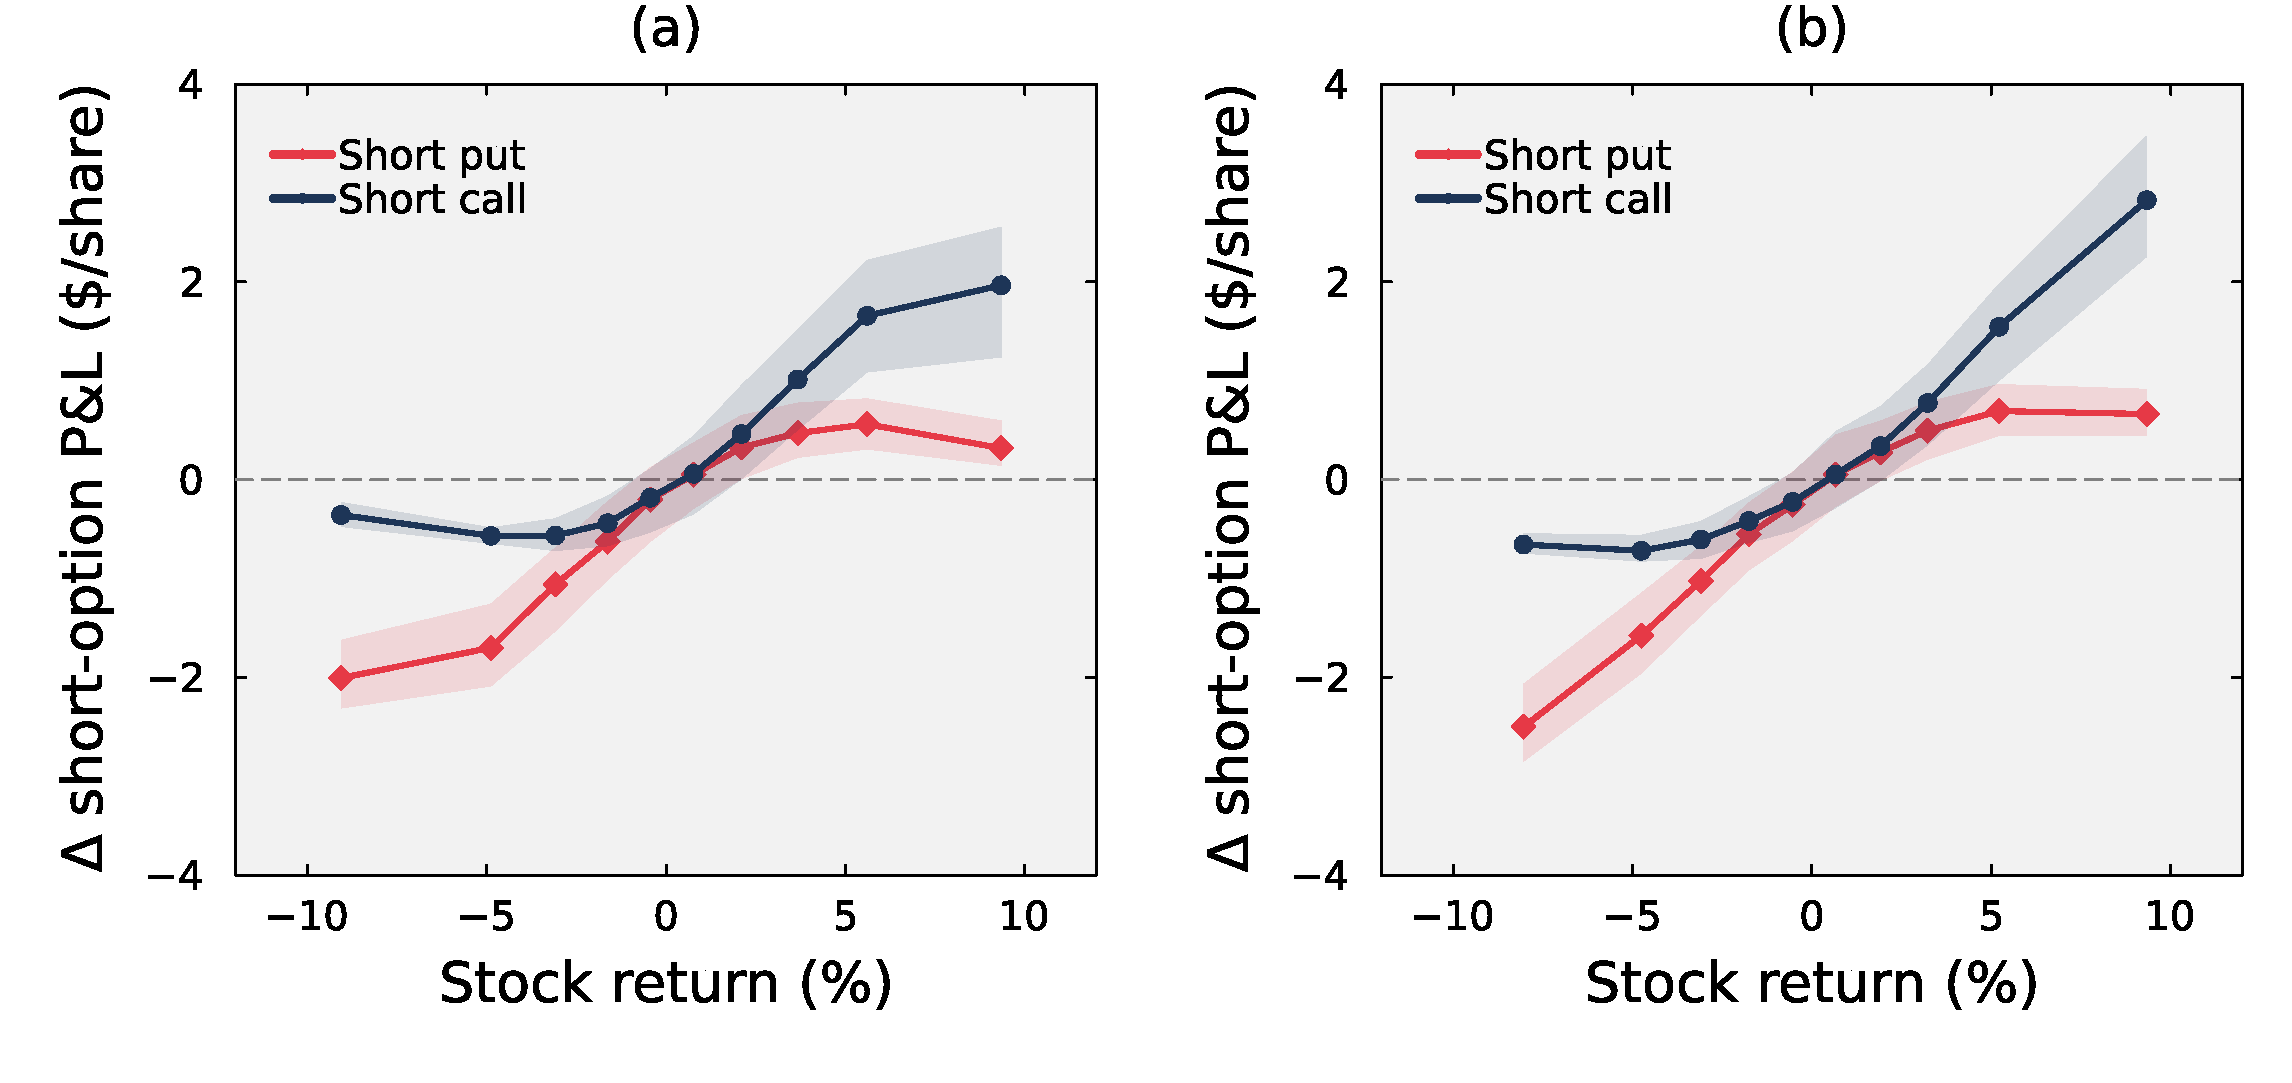
\includegraphics[width=\textwidth]{sections/figures/dynamic_ablation.pdf}
\caption{Effect of linking IV shocks to stock returns on short-option P\&L before expiration, by stock return, after ten trading days for (a) GS and (b) LLY. Each difference is full-factor P\&L ($\rho=-0.6$) minus uncoupled-factor P\&L ($\rho=0$) on the same stock path, with the same independent normal shocks. Negative values indicate worse short-position P\&L under coupling. The 3{,}000 paths per ticker are sorted by stock return and divided into ten groups of 300. Symbols show each group's median P\&L difference at its median stock return, and lines connect the symbols. Shaded bands span each group's 25th--75th percentiles. These bands describe variation across paths, not confidence intervals. Red circles denote puts and navy diamonds denote calls. All prices are evaluated on May 12, 2026, with 17 calendar days to expiration.}\label{fig:dynamic_ablation}
\end{figure}

We then refined the tree and compared prices across strikes, and found that the variant differences exceeded numerical error but that some GS prices violated necessary strike conditions (Supplementary Tables~\ref{tab:ablation_seeds} and~\ref{tab:strike_audit}). Increasing the tree from 201 to 401 steps changed sampled prices by at most \$0.0017 per share (Supplementary Table~\ref{tab:ablation_seeds}). That change was more than two orders of magnitude below the mean absolute differences among IV variants (Supplementary Table~\ref{tab:dynamic_ablation}). No factor reached the variance floor in the four scenario options (Supplementary Table~\ref{tab:ablation_seeds}). However, strike/spot left the training interval on 0.7--2.9\% of path dates before expiration, across tickers, options, and seeds. On those dates, prices used extrapolated surface values (Supplementary Table~\ref{tab:ablation_seeds}). Each convexity violation corresponds to a butterfly spread priced below zero. At 401 steps, the GS direct surface exceeded the \$0.01 convexity tolerance in 178 of 1{,}818 tested strike triples, and the largest excess was \$0.113 per share (Supplementary Table~\ref{tab:strike_audit_depth}). The GS full factor had three monotonicity violations among 2{,}020 adjacent-strike comparisons, with a maximum of \$0.013 (Supplementary Table~\ref{tab:strike_audit_depth}). These violations appeared at both tree depths (Supplementary Table~\ref{tab:strike_audit_depth}). No LLY variant violated the tested conditions at the stated tolerance. Pricing each option accurately on its own therefore did not make the GS prices consistent across strikes.
\FloatBarrier
